\documentclass[tikz]{standalone}

\usetikzlibrary{calc}
\usetikzlibrary{shapes}

\definecolor{c1}{RGB}{62,91,90}
\definecolor{c2}{RGB}{103,152,149}
\definecolor{c3}{RGB}{194,214,213}

\begin{document}
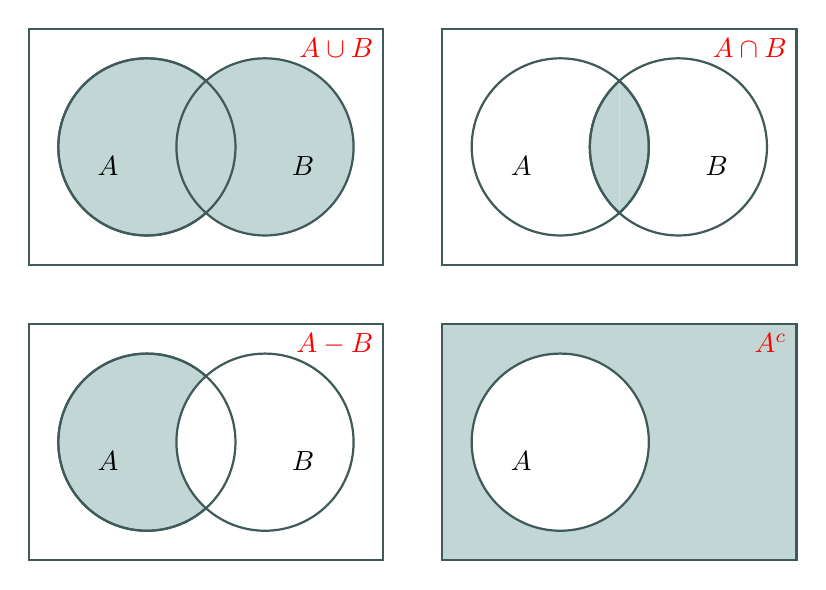
\begin{tikzpicture}[scale=1.5]
    \begin{scope} %union
        \draw[draw=c1,thick] (0,0) rectangle (3,2);
        \draw[draw=c1,thick,fill=c3] (1,1) circle (0.75);
        \draw[draw=c1,thick,fill=c3] (2,1) circle (0.75);
        % the second circle filled hides a part of the first circle
        % that's why we need to draw again the 1st circle, but no fill!
        \draw[draw=c1,thick] (1,1) circle (0.75);
        \node[below right] at (0.5,1) {$A$};
        \node[below left] at (2.5,1) {$B$};
        \node[below left,red ] at (3,2) {$A \cup B$};
    \end{scope}
    % second picture, shift to the right 3.5 cm, bigger than the bounding rectangle (3,2)
    \begin{scope}[xshift=3.5cm] %intersection
        \draw[draw=c1,thick] (0,0) rectangle (3,2);
        % using scope and clip: scope to limit the clipping
        % clipping: outside the clipped area not visible     
        \begin{scope} % this is for the right part of the intersection moon
        \clip (1.5,0) rectangle (3,2);
        \draw[draw=c1,thick,fill=c3] (1,1) circle (0.75);
        \end{scope}
        \begin{scope} % this is for the left part of the intersection moon
        \clip (0,0) rectangle (1.5,2);
        \draw[draw=c1,thick,fill=c3] (2,1) circle (0.75);
        \end{scope}
        % now draw the circles for sets A and B
        \draw[draw=c1,thick] (1,1) circle (0.75);
        \draw[draw=c1,thick] (2,1) circle (0.75);
        \node[below right] at (0.5,1) {$A$};
        \node[below left] at (2.5,1) {$B$};
        \node[below left,red ] at (3,2) {$A \cap B$};
    \end{scope}
    % this is the 3rd pic, below the 1st pic, so yshifted =-2.5cm
    \begin{scope}[yshift=-2.5cm] %difference
        \draw[draw=c1,thick] (0,0) rectangle (3,2);
        \draw[draw=c1,thick,fill=c3] (1,1) circle (0.75);    % this circle for set A
        \draw[draw=c1,thick,fill=white] (2,1) circle (0.75); % fill white to hide part of A
        \draw[draw=c1,thick] (1,1) circle (0.75);            % then redraw A
        \node[below right] at (0.5,1) {$A$};
        \node[below left] at (2.5,1) {$B$};
        \node[below left,red ] at (3,2) {$A - B$};
    \end{scope}

    \begin{scope}[xshift=3.5cm,yshift=-2.5cm] %complement
        \draw[draw=c1,thick,fill=c3] (0,0) rectangle (3,2);
        \draw[draw=c1,thick,fill=white] (1,1) circle (0.75);
        %\draw[draw=c1,thick] (2,1) circle (0.75);
        \node[below right] at (0.5,1) {$A$};
        \node[below left,red] at (3,2) {$A^c$};
    \end{scope}
\end{tikzpicture}
\end{document}

